\chapter{Application}\label{D:application}

This chapter aims to develop the tasks introduced for the application layer in this project Gantt (see figure \ref{F:tpgp}).

\section{REST API}

As previously said, it's required to develop an API ready to be used over cloud environments in order to ease creating specific and new applications over the LMS framework.

The common and widely used format for cloud services intercommunication is JSON, as it is also used for the TCP socket API of the LMS framework. Then, it's recommended to follow this premise as much as possible.

A suitable technology to work with JSON formatted messages which widely known for its good performance is Node.js (--REFERENCE--). Node.js is an open source, cross-platform runtime environment for server-side and networking applications. It provides an event-driven architecture and a non-blocking I/O API that optimizes application's throughput and scalability. This technology is commonly used for real-time web applications. 

Moreover, working with Node.js means avoiding serialization of the JSON messages by increasing services intercommunication performance (i.e.: less computational cost and less processing time). A Node.js key point is also the fact of not requiring specific HTTP servers in order to serve the application itself.

Then, the common Noje.js framework for developing web applications and REST APIs is Express.js (--REFERENCE--). It's the de facto standard server framework for Node.js. The middleware is going to use its routing system, which refers to the definition of end points (URIs with HTTP request methods like GET, POST, PUT and DELETE) to an application and how it responds to client requests.

Following is the proposed software structure for developing the RESTfull API middleware (responsible to translate to the TCP socket API of the LMS framework):

\begin{figure}[!htb]
\begin{center}
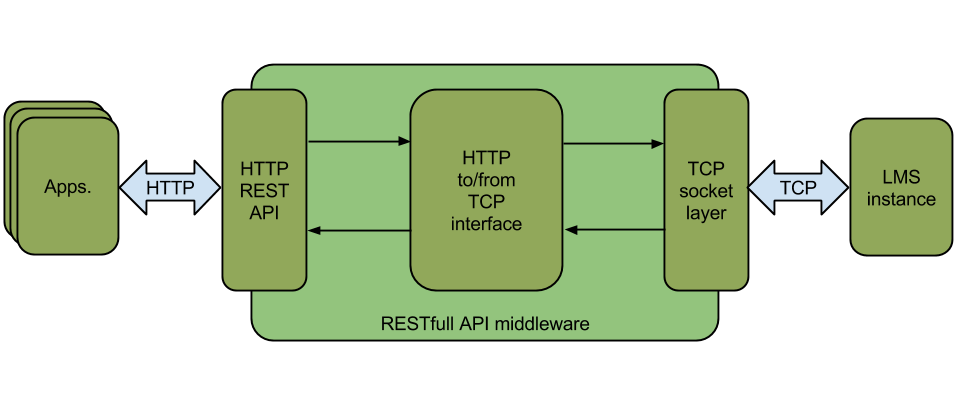
\includegraphics[width=1\textwidth]{./images/RESTAPI.png}
\caption{RESTfull API middleware architecture}
\label{F:restAPI}
\end{center}
\end{figure}

\begin{itemize}
\item The HTTP REST API layer \hfill

This layer is the one that is waiting for the HTTP queries from external applications. It implements required routes to handle specific HTTP queries. First implementation will not implement multi LMS management but single. As shown in figure \ref{F:restAPI}.

\item The interface layer \hfill

This layer handles the body messages from the previous layer's HTTP queries and manipulates them in order to create an as much generic as possible API by adapting the messages to be sent through next layer.

\item The TCP socket layer \hfill

This layer is the responsible to send and receive JSON formatted TCP socket messages between the LMS targeted instance.
\end{itemize}

As introduced in section {SOA:LMSframework} and deeply explained in ANNEX XX, there are two different management layers: the generic and the filter specific. So, proposed API's structure to be implemented is as shown next:

\begin{itemize}
\item Generic management queries
\begin{itemize}
\item Connect \hfill

Checks if an existing instance of LMS is running and sets the LMS port and LMS host to work with.
\begin{quote}
\begin{verbatim}
POST http://<host>:<port>/api/connect
JSON    {
            "port":<lms-port>,
            "host":"<lms-host>"
        }
\end{verbatim}
\end{quote}
\item Disconnect \hfill

Resets the running LMS instance and sets \verb|lms-port| and \verb|lms-host| to null in order to connect again to the same or any another LMS instance running.
\begin{quote}
\begin{verbatim}
GET http://<host>:<port>/api/disconnect
\end{verbatim}
\end{quote}
\item State \hfill

Gets the state object of the current LMS instance connected to (JSON object with the configured filters and paths).
\begin{quote}
\begin{verbatim}
GET http://<host>:<port>/api/state
\end{verbatim}
\end{quote}
\item Create a filter \hfill

Creates a filter (current types are: receiver, transmitter, demuxer, dasher, audioDecoder, audioEncoder, videoDecoder, videoResampler, videoEncoder, audioMixer, videoMixer) with an unique identifier.
\begin{quote}
\begin{verbatim}
POST http://<host>:<port>/api/createFilter
JSON    {
            "id": filterID,
            "type": "type"
        }
\end{verbatim}
\end{quote}        
\item Create a path of filters \hfill

Create a path of filters. A path can be a master path or an slave one, as shown:

\begin{itemize}

\item Master path
\begin{quote}
\begin{verbatim}
POST http://<host>:<port>/api/createPath
JSON    { 
            'id' : pathId, 
            'orgFilterId' : orgFilterId, 
            'dstFilterId' : dstFilterId, 
            'orgWriterId' : orgWriterId, 
            'dstReaderId' : dstReaderId, 
            'midFiltersIds' : [filterID1, filterID2,...] 
        }
\end{verbatim}
\end{quote}
\item Slave path of previous master path
\begin{quote}
\begin{verbatim}
POST http://<host>:<port>/api/createPath
JSON    { 
            'id' : pathId, 
            'orgFilterId' : filterID1, 
            'dstFilterId' : dstFilterId2, 
            'orgWriterId' : -1, 
            'dstReaderId' : dstReaderId2, 
            'midFiltersIds' : [filterID3, filterID4,...] 
        }  
\end{verbatim}
\end{quote}
\end{itemize}
\end{itemize}
\item Specific filter management queries        
\begin{itemize}
\item Configure an existing filter \hfill

Configures an existing filter (each filter has its own actions defined, check ANNEX XXX)
\begin{quote}
\begin{verbatim}
PUT http://<host>:<port>/api/filter/:filterID
JSON    [
            {
                "action":"the action",
                    "params":{
                        "param1":param1,
                        "param2":"param2",
                        "param3":"param3",
                        "param4":true
                }
            }
        ]
\end{verbatim}
\end{quote}

\end{itemize}
\end{itemize}

So, with previous API proposal, the whole TCP socket API becomes simplified.

Moreover, specific responses format to client has been proposed as shown:

\begin{itemize}
\item Success messages \hfill

It may be a string, bool, array or another object, depending on the request method

\begin{quote}
\begin{verbatim}
JSON    {
            "message": { the incoming message }
        }
\end{verbatim}
\end{quote}        
\item Error messages \hfill

\begin{quote}
\begin{verbatim}
JSON    {
            "error": "the error message"
        }
\end{verbatim}
\end{quote}
\end{itemize}

Finally, in order to know how this structure is implemented in the middleware application check ANNEX XXX to see the code.

\section{Input network metrics}



\section{Output network metrics}



\section{Frame delay metrics}



\section{Frame losses metrics}




-> ENGANXAR CORREU ROSS

-> DIR Q RESTFUL API MIDDLEWARE TRADUEIX HTTP TO TCP (afegint architecture REST per a assegurar que s'aplica un estic d'arquitectura de software escalable per al nuvol.